\documentclass[11pt]{article}
%Gummi|065|=)
\title{\textbf{CS 374 Spring 2018 \\
				Homework 2}}
\author{Nathaniel Murphy (njmurph3) \\
		Tanvi Modi (tmodi3) \\
		Marianne Huang (mhuang46)}
\date{}
\usepackage{a4wide}
\usepackage{amsmath}
\usepackage{amsthm}
\usepackage{amssymb}
\usepackage{mathtools}
\usepackage{tikz}
\usetikzlibrary{automata,positioning}

\begin{document}

\maketitle

\section*{Problem 3 Solution:}
*NOTE* The following NFA is not in any way a mathematical definition. It is solely a visual aide. The formal definition of the NFA for language $T_k$ can be found on the next page.  
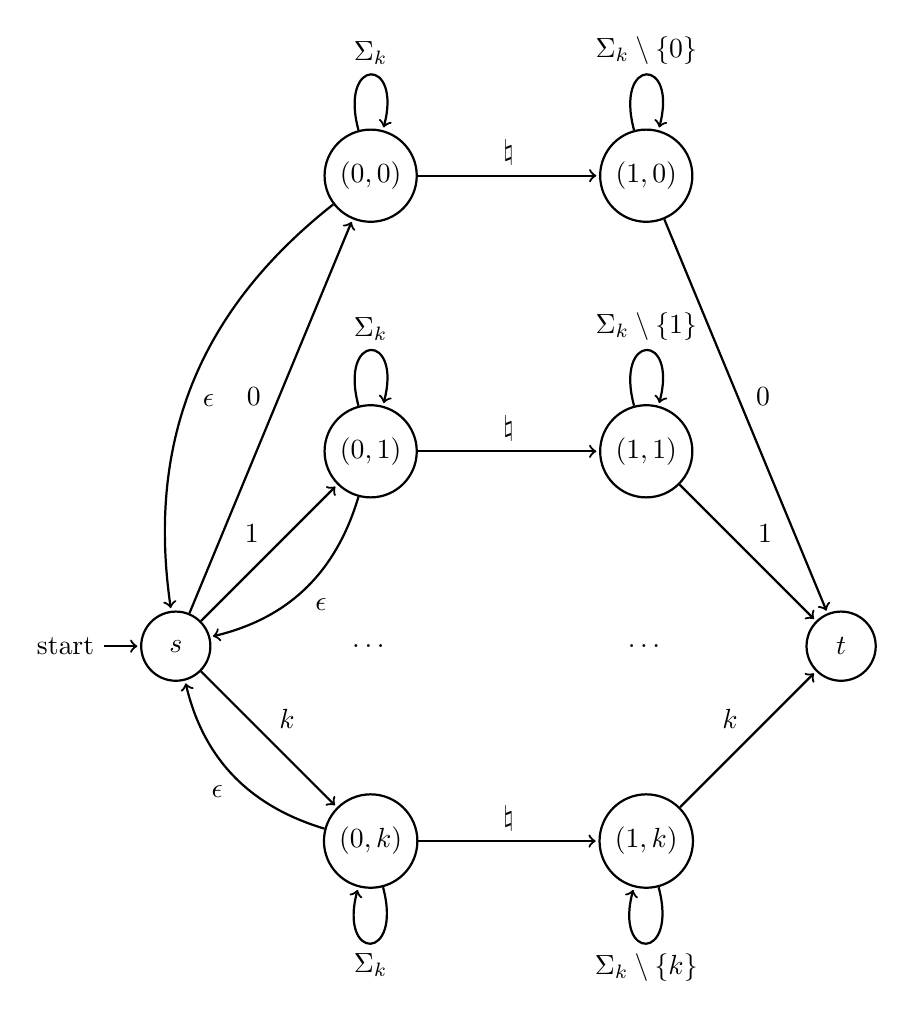
\begin{tikzpicture}[->,shorten >=1pt, auto, on grid, node distance=3.5cm, thick, node/.style={circle,draw}]
	\node[state,initial] (qs) {$s$};
	\node[state] (q1) [above right=of qs] {$(0,1)$};
	\node[state] (q0) [above=of q1] {$(0,0)$};
	\node[state] (qk) [below right=of qs] {$(0,k)$};
	\node[state] (qq0)[right=of q0] {$(1,0)$};
	\node[state] (qq1)[right=of q1] {$(1,1)$};
	\node[state] (qqk)[right=of qk] {$(1,k)$};
	\node[state] (t)  [above right=of qqk] {$t$};
	\path (qs) edge node {0} (q0);
	\path (qs) edge node {1} (q1);
	\path (qs) edge node {$k$} (qk);
	\path (q0) edge[bend right] node {$\epsilon$} (qs);
	\path (q1) edge[bend left] node {$\epsilon$} (qs);
	\path (qk) edge[bend left] node {$\epsilon$} (qs);
	\path (q1) -- node[auto=false]{\ldots} (qk);
	\path (qq1) -- node[auto=false]{\ldots} (qqk);
	\path (q0) edge node {$\natural$} (qq0);
	\path (q1) edge node {$\natural$} (qq1);
	\path (qk) edge node {$\natural$} (qqk);
	\path (q0) edge [loop above] node {$\Sigma_k$} ();
	\path (q1) edge [loop above] node {$\Sigma_k$} ();
	\path (qk) edge [loop below] node {$\Sigma_k$} ();
	\path (qq0) edge [loop above] node {$\Sigma_k\setminus\{0\}$} ();
	\path (qq1) edge [loop above] node {$\Sigma_k\setminus\{1\}$} ();
	\path (qqk) edge [loop below] node {$\Sigma_k\setminus\{k\}$} ();
	\path (qq0) edge node {0} (t);
	\path (qq1) edge node {1} (t);
	\path (qqk) edge node {$k$} (t);
\end{tikzpicture}

\newpage

\subsection*{}
Let us define NFA $N=(Q,\Sigma,\delta,s,A)$ such that $N$ defines the language $T_k$
\begin{itemize}
	\item $Q=\{0, 1\} \times \Sigma_k \cup\{t,S\}$, where $2^k$ is the set of all binary strings of length k 
	\item $\Sigma=\Sigma_k$
	\item $s=\{S\}$
	\item $A=\{t\}$
	\item $\delta$ is defined as follows \\ \[\delta(q,a)=\begin{cases}
		\{S, (0,a)\} & \text{if }q=S \\
        \{(0, j)\} & \text{if }q=(i, j)\text{ where }i=0\text{ and }j\in\Sigma_k^* \\
		\{(1,j)\} & \text{if }q=(i, j)\text{ where }i=0\text{ and }a=\natural \\
		\{(1,j)\} & \text{if }q=(i, j)\text{ where }i=1\text{ and }a\neq j \\
		\{t\} & \text{if }q=(i, j)\text{ where }i=1\text{ and }a=j \\
	\end{cases}\]
\end{itemize}
Reading an input symbol $a$ from the start state $S$ where $a \in\Sigma_k$ will bring the existing thread to state $a$ where the $i=0$ denotes a $\natural$ has not been seen yet. It will also activate a new thread in $S$ due to an $\epsilon$ transition. It will stay in the state $(0, j)$ if it continues to read input symbols $j\in \Sigma_k^*$ but has not yet read $\natural$.
If $i=1$, the $\natural$ symbol has been read. Then, if $a\neq j$ that were seen before $\natural$, it stays in that state. It moves to an accept state $\{t\}$ if $i=1$ and it reads an input $a=j$ that is in the set of symbols seen before $\natural$.
\end{document}